
\chapter{Thématique}


\section{Modélisation des systèmes biologiques}\label{sec:model}
Les réseaux de régulation biologique (RRB \label{sec:RRB}) sont généralement représentés par des graphes d'interactions(La figure \ref{fig:exRRB} donne un exemple de Réseau de Régulation Biologique simple). 
De nombreux modèles mathématiques et informatiques ont été proposés
pour l'ananlyse et la compréhension de la dynamique de ces réseaux. Les approches de modélisation continue se font par des équations différentielles. A chaque composant est 
associé une variable continue qui détermine son influence sur sa cible. Cette approche est difficilement utilisable sur des RRB de grande taille de part l'introduction de nombreux 
paramètres inconnus et généralement difficiles à obtenir à partir de la littérature et des expérimentations. L'introduction de modèles discrets ou qualitatifs permet de contourner cette difficulté. En effet, plutôt que de considérer 
les valeurs réelles de concentration des protéines synthétisées, Thomas propose dans son modèle introduit en 1973 \cite{Thomas73}, de se servir des seuils qui représentent des 
valeurs de ces concentrations au-delà desquelles les influences entre composants évoluent. Afin de représenter plus finement la dynamique discrète des RRB, des notions de délais et de 
stochasticité ont été introuduites sur les interactions. Plusieurs approches dites hybrides(continues,discrètes) ont été proposées pour répondre à ce besoin. La plupart de ces méthodes souffre d'une 
du phénomène d'explosion combinatoire sur le graphe d'états du système qui les rend difficilement utilisables sur des réseaux au delà de $20$ gènes.

La modélisation en frappe de processus \cite{PMR10-TCSB,PaulevePhD} qui est un formalisme inspiré du $\pi-calcul$ Stochastique, à laquelle est adjointe une compositionalité importante, permet
d'éviter un recours à un dépliage coûteux du graphe d'état. Cependant, l'inférence de paramètres dans un espace continu reste encore très coûteuse. Heureusement, la disponibilité 
des données des séries temporelles issues des expériences, nous permet d'envisager une intégration formelle des notions de délais dans de grands modèles Hybrides. 

\section{Intégration des données temporelles dans un RRB}
La problématique de l'intégration des informations temporelles issues des séries temporelles dans les modèles a déjà été abordée avec des approches différentes. Nous pouvons 
citer les approches basées sur l'utilisation des équations différentielles \cite{batt2005validation,mobashir2012simulated,tyson2003sniffers}, les méthodes basées sur l'utilisation
des approches stochastiques \cite{macnamara2012state} et des méthodes basées sur l'intégration efficiente et complète des données dans les modèles à large échèlles \cite{guziolowski2013exhaustively,mitsos2009identifying}.

Aussi, nous comptons nous servir du formalisme des frappes de processus pour apporter une contribution à l'intégration des informations temporelles dans les modèles hybrides.
En effet, le formalisme des frappes de processus demande deux paramètres pour la simulation stochastique. Le taux généralement noté $r$ et un facteur d'absorption de 
stochasticité noté $sa$. Nous allons également nous servir des données de séries temporelles dont la disponibilté n'est plus un réel défi grâce à l'évolution technologique
pour estimer les informations temporelles des composants du réseau. Nous pensons ainsi pouvoir proposer une méthode automatique de génération de grands réseaux de régulation
biologique dans le formalisme des frappes de processus, auxquels nous avons intégré des informations sur les délais et l'aléatoire.


Nous comptons appliquer nos méthodes à l'étude de la différentiation des cellules de la peau. En effet un modèle préliminaire discret de ce système  a été obtenu et étudié 
dans de precédents travaux \cite{guziolowski2012automatic}. De plus, dans le cadre d'une collaboration avec le Centre Allemand de Recherche contre le Cancer à Heidelberg, nous pouvons accéder à des études
publiées et non-publiées fournissant des données de séries temporelles sur ce système.


\begin{figure}[h]
\begin{minipage}{0.4\linewidth}
\centering
\scalebox{1.1}{
\begin{tikzpicture}[grn]
\path[use as bounding box] (0,-0.7) rectangle (3.5,0.7);
\node[inner sep=0] (a) at (2,0) {a};
\node[inner sep=0] (b) at (0,0) {b};
\node[inner sep=0] (c) at (3.5,0) {c};
%\path
%  node[elabel, below=-1em of a] {$0..2$}
%  node[elabel, below=-1em of b] {$0..1$}
%  node[elabel, below=-1em of c] {$0..1$};
\path[->]
  (b) edge[bend right] node[elabel, below=-3pt] {$+1$} (a)
  (c) edge node[elabel, above=-5pt] {$+1$} (a)
  (a) edge[bend right] node[elabel, above=-5pt] {$-2$} (b);
\end{tikzpicture}
}
\end{minipage}
\begin{minipage}{0.6\linewidth}
\centering
\begin{align*}
K_{a,\{b,c\},\emptyset} &= 2 & K_{b,\{a\},\emptyset} &= 1 \\
K_{a,\{b\},\{c\}} &= 1 & K_{b,\emptyset,\{a\}} &= 0 \\
K_{a,\{c\},\{b\}} &= 1 &&\\
K_{a,\emptyset,\{b,c\}} &= 0 & K_{c,\emptyset,\emptyset} &= 1
\end{align*}
\end{minipage}
\caption{\label{fig:exRRB}
Exemple de Réseau de Régulation Biologique, comprenant un Graphe des Interactions (à gauche) et une paramétrisation (à droite).
Chaque nœud du graphe représente un composant et chaque arc une régulation
dont l'étiquette indique le type (“$+$” pour une activation et “$-$” pour une inhibition) et le seuil.
Les paramètres tiennent lieu de points focaux pour l'état concerné.
}
\end{figure}


\section{Données}

Dans cette première section, nous présentons les données qui nous ont servi de support pour la modélisation de notre système. 
Nous allons nous focaliser sur deux éléments principaux: le graphe des interactions qui décrit les composants du système avec 
les différentes interactions qui existent entre ces composants et les données d'expressions des gènes. 


\subsection{Le graphe des interactions}
Le graphe d'interactions qui décrit le processus de différentiation cellulaire est un réseau de signalisation qui spécifie 
les composants et les interactions entre les différents composants. C'est un large réseau qui compte près de $200$ composants(molécules ou sommet intermédiaires) 
et à peu près $400$ interactions entre ces composants. 
Les composants sont des noeuds qui peuvent être les gènes, les protéines, les complexes et les indicateurs d'états cellulaires.
Les interactions entre les composants sont de plusieurs natures. Nous avons principalement les activations entre composants, les inhibitions,
les décompositions de complexes. Le réseau est activé par une stimulation au Calcium d'un noeud principal appelé E-cardherin. Ce noeud est considéré 
comme noeud d'entré du réseau. C'est à partir de lui que va partir les principaux signaux qui vont se propager dans le réseau. A côté du noeud 
principal E-cardherin, nous avons les protéines de signalisations qui auront la propriété de s'activer et de se désactiver une fois qu'elles reçoivent un  
signal d'activation ou d'inhibition. Le graphe d'interaction contient aussi des gènes qui sont particuliés parce qu'ils sont considérés comme 
les sorties du réseau et leur expression a pu être mesurée tout au long de l'expérience. Le dernier type de noeud que nous avons dans le réseau sont 
les noeuds qui nous donnent les états cellulaires. 

% insérer le graphe qui représente le réseau 


\subsection{Les données de séries temporelles}

Les données de séries temporelles dont nous disposons  sont les données obtenues après une expérience réelle en laboratoire. Ces données sont les réponses d'une simulation 
du noeud d'entrée du réseau E-cardherin au calcium, mesurées sur certains gènes en sortie. Nous avons un total de $200$ gènes dont nous avons pu observer la dynamique tout au long 
de l'expérience. Nous avons retenu $12$ transcrits en raison de leur dynamique. La figure \ref{fig:12genes} est un graphique de la dynamique des
$12$ gènes que nous avons sélectionné. L'expérience dure $24$ heures. Pendant les $10$ premières heures, nous observons une forte activité des gènes à travers 
les dynamiques des courbes d'expressions. Cette forte activité est marquée par l'atteinte des pics d'expressions pour tous les gènes.  

\begin{figure}[p]
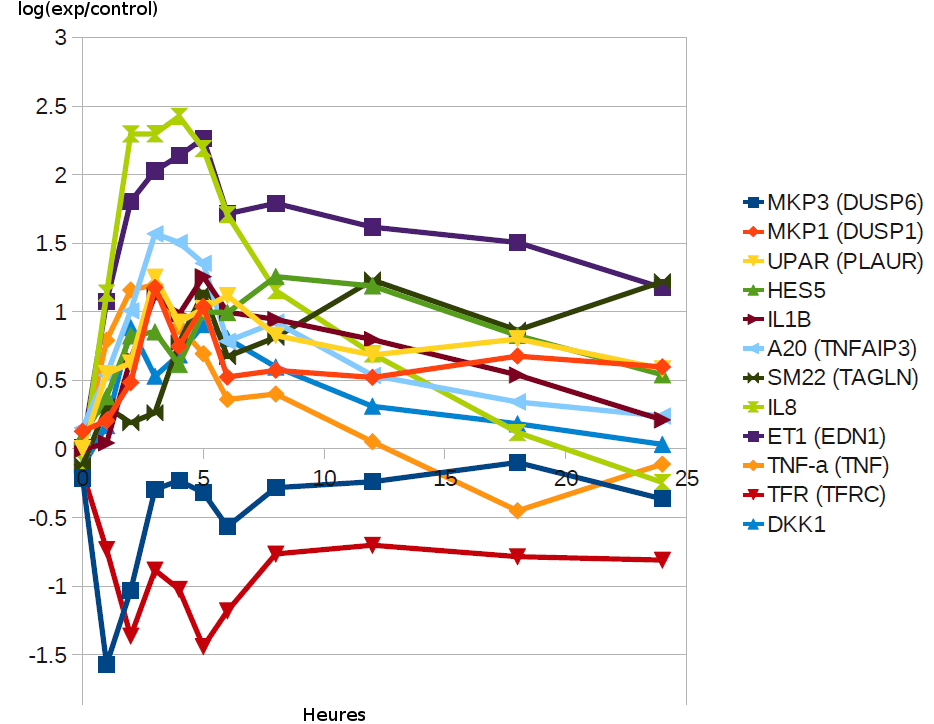
\includegraphics[scale=0.5]{images/12genes.png}
\caption{\label{fig:12genes}
Données de séries temporelles des gènes du réseau.
}
\end{figure}


\section{Process Hitting}\label{sec:PH}
Une façon de modéliser des Réseaux de Régulation Biologiques à l'aide de $\pi$-calcul, appelée Process Hitting (ou Frappes de Processus), a été récemment introduite par l'équipe MeForBio
dans \cite{PMR10-TCSB,PaulevePhD}.
Elle propose un point de vue plus modulable des influences entre composants grâce à une représentation d'actions atomiques entre ceux-ci.
Cette représentation particulière offre des possibilités d'analyse statique efficaces permettant de sur-approximer et sous-approximer l'atteignabilité d'un processus \cite{PMR12-MSCS}.
De plus, son atomicité permet d'adopter différents niveaux d'abstraction dans la modélisation, afin notamment de représenter une sur-approximation du comportement d'un système dont la spécification des coopérations ne serait pas entièrement déterminée.
Une méthode efficace de détermination des points fixes a aussi été développée.
La figure \ref{fig:exPH} donne un exemple de Process Hitting.

Plusieurs extensions ont aussi été proposées pour enrichir ce formalisme.
Une première repose sur l'introduction de la stochasticité afin de modéliser la durée d'évolution relative des composants à l'aide des probabilités.
Cette extension nécessite une simulation de l'exécution du modèle afin d'en extraite des propriétés empiriques, ou l'utilisation d'un model checker.
Une seconde extension consiste en l'attribution de classes de priorités aux actions, afin d'imposer formellement un ordre de tir entre celles-ci.
Cette sémantique reposant sur des priorités fixes permet de modéliser des comportements plus fins, par exemple au niveau des coopérations.
Elle ne modifie pas les résultats concernant la recherche de points fixes.

\begin{figure}[h]
\centering
\scalebox{1.1}{
\begin{tikzpicture}
\path[use as bounding box] (-2,-5.2) rectangle (7,0.7);

\TSort{(0,0)}{b}{2}{t}
\TSort{(0,-3.8)}{c}{2}{b}
\TSort{(4.5,-3)}{a}{3}{r}

\TSetTick{bc}{0}{00}
\TSetTick{bc}{1}{01}
\TSetTick{bc}{2}{10}
\TSetTick{bc}{3}{11}
% \TSetSortLbcel{bc}{$\neg a\wedge b$}
\TSort{(-0.5,-2)}{bc}{4}{b}

\THit{b_1}{bend right}{bc_0}{.north}{bc_2}
\THit{b_1}{bend right}{bc_1}{.north}{bc_3}
\THit{b_0}{}{bc_2}{.north west}{bc_0}
\THit{b_0}{}{bc_3}{.north west}{bc_1}

\THit{c_0}{}{bc_1}{.south}{bc_0}
\THit{c_0}{}{bc_3}{.south}{bc_2}
\THit{c_1}{}{bc_0}{.south}{bc_1}
\THit{c_1}{}{bc_2}{.south}{bc_3}

\path[bounce, bend right=25]
\TBounce{bc_2}{}{bc_0}{.north east}
\TBounce{bc_3}{}{bc_1}{.north east}
;
\path[bounce, bend left=80, distance=30]
\TBounce{bc_0}{}{bc_2}{.north}
\TBounce{bc_1}{}{bc_3}{.north}
;
\path[bounce, bend right]
\TBounce{bc_0}{}{bc_1}{.west}
\TBounce{bc_2}{}{bc_3}{.west}
;
\path[bounce, bend left]
\TBounce{bc_3}{}{bc_2}{.east}
\TBounce{bc_1}{}{bc_0}{.east}
;

\THit{bc_3}{thick}{a_1}{.north west}{a_2}
\THit{bc_0}{thick,bend right=130, in=305, distance=140}{a_1}{.south east}{a_0}
\path[bounce, bend left=40]
\TBounce{a_1}{thick}{a_2}{.south west}
\TBounce{a_1}{thick}{a_0}{.north east}
;

\THit{b_0}{thick,bend left,out=50,in=150}{a_2}{.west}{a_1}
\THit{b_1}{thick,bend left,out=80,in=70,distance=100}{a_0}{.east}{a_1}
\path[bounce]
\TBounce{a_2}{thick,bend right=40}{a_1}{.west}
\TBounce{a_0}{thick,bend right=40}{a_1}{.east}
;

\THit{c_0}{thick,bend left,out=270,in=290, distance=115}{a_2}{.east}{a_1}
\THit{c_1}{thick}{a_0}{.north west}{a_1}
\path[bounce]
\TBounce{a_2}{thick,bend left=40}{a_1}{.north east}
\TBounce{a_0}{thick,bend left=40}{a_1}{.south west}
;

\THit{a_2}{bend left, out=290, in=120}{b_1}{.south}{b_0}
\path[bounce, bend left]
\TBounce{b_1}{}{b_0}{.south}
;

\end{tikzpicture}
}

\caption{\label{fig:exPH}
Exemple de Process Hitting comprenant quatre sortes : $a$, $b$, $c$ et $bc$.
La sorte $bc$ est appelée sorte coopérative (cf. section \ref{sec:PH}).
}
\end{figure}



